\documentclass[conference]{IEEEtran}

% ========= パッケージ =========
\usepackage{cite}
\usepackage{amsmath,amssymb}
\usepackage{siunitx}
\usepackage{graphicx}
\usepackage[caption=false,font=footnotesize]{subfig}
\usepackage{booktabs}
\usepackage{tikz}
\usetikzlibrary{positioning,arrows.meta}
\usepackage{newtxtext,newtxmath}
\usepackage[hidelinks]{hyperref}
\usepackage{stfloats}
\usepackage[section]{placeins}   % 図表を節内に固定

% ========= 記号マクロ =========
\newcommand{\Vth}{V_{\mathrm{th}}}
\newcommand{\Ea}{E_{\mathrm{a}}}
\newcommand{\betaW}{\beta}
\newcommand{\etaW}{\eta}
\sisetup{detect-all, per-mode=symbol, separate-uncertainty = true}

% ========= 体裁調整 =========
\setlength{\textfloatsep}{9pt plus 2pt minus 2pt}
\setlength{\floatsep}{7pt plus 2pt minus 2pt}
\setlength{\intextsep}{6pt plus 2pt minus 2pt}
\setlength{\abovecaptionskip}{3pt}
\clubpenalty=10000
\widowpenalty=10000

\newcommand{\figw}{0.90\linewidth}

% ========= タイトル =========
\begin{document}

\title{Low-Cost Integration of 1.8-V FeFET on 0.18-$\mu$m CMOS:\\
+1 Mask and a Single ALD Tool, with Reliability Assessment}

\author{\IEEEauthorblockN{Shinichi Samizo}
\IEEEauthorblockA{Independent Semiconductor Researcher\\
Former Engineer at Seiko Epson Corporation\\
Email: shin3t72@gmail.com\quad GitHub: \url{https://github.com/Samizo-AITL}}
}

\maketitle

% ========= Abstract =========
\begin{abstract}
Ferroelectric FETs (FeFETs) are promising CMOS-compatible embedded nonvolatile memories. 
This paper demonstrates a 1.8~V FeFET module integrated on a legacy 0.18~$\mu$m CMOS process with only one additional mask and a single ALD tool. 
Fabricated devices show endurance exceeding $10^5$ program/erase cycles and retention longer than 10 years at 85$^\circ$C. 
Reliability was characterized on FeCAP/FeFET structures, including time-zero dielectric breakdown (TZDB), time-dependent dielectric breakdown (TDDB), endurance, and retention. 

Unlike approaches aiming for high-density NVM, our concept employs FeFETs as a supplementary backup for SRAM, avoiding aggressive scaling and thus improving yield and reliability. 
The method offers a cost-effective path to extend mature-node lifetimes and to enable dependable embedded NVM for automotive, industrial, and IoT applications, while high-temperature retention remains the key limiter.
\end{abstract}

% ========= Introduction =========
\section{Introduction}
Ferroelectric Hf$_{0.5}$Zr$_{0.5}$O$_2$ (HZO) thin films have emerged as a leading candidate for CMOS-compatible nonvolatile memories (NVMs), 
offering low-voltage operation, scalability, and compatibility with standard CMOS thermal budgets~\cite{boscke2011,mueller2012,mikolajick2019,mueller2015}.
Compared with embedded flash (eFlash), FeFETs provide lower process cost and superior scalability; 
unlike MRAM and ReRAM, they require no exotic materials or additional BEOL steps, making them highly attractive for embedded integration.

While much prior research targets sub-28~nm advanced nodes, mature nodes such as 0.18~$\mu$m remain workhorses in automotive and industrial electronics, 
where cost efficiency, process maturity, and long supply lifetimes are essential.  
In this context, FeFETs are not positioned as a high-density replacement memory, but rather as a \textit{supplementary backup to SRAM}, 
which avoids aggressive scaling, improves yield, and enhances reliability.

\textbf{This work makes four contributions:}  
(i) demonstration of a +1 mask, low-cost FeFET module on a 0.18~$\mu$m baseline CMOS process,  
(ii) realization using only a single ALD chamber for Al$_2$O$_3$/HZO and a standard TiN gate process,  
(iii) proposal of a yield- and reliability-friendly \textit{SRAM+FeFET} backup/restore system model, and  
(iv) comprehensive reliability characterization (time-zero dielectric breakdown (TZDB), time-dependent dielectric breakdown (TDDB), endurance, and retention) on FeCAP/FeFET structures.

\FloatBarrier

% ========= Process Integration =========
\section{Process Integration}
Baseline is a 0.18~$\mu$m CMOS platform (1.8~V core, optional 3.3~V I/O).
The FeFET module is inserted \textbf{after Co-salicide (RTA)}, requiring only one additional mask.
The HZO/Al$_2$O$_3$ ferroelectric stack is deposited by a single ALD tool (both interlayer Al$_2$O$_3$ and HZO in one chamber), 
and the TiN metal gate is formed by collimated or long-throw PVD sputtering.
This integration minimizes line modification and suppresses capital expenditure.

\subsection{Process Flow}
\begin{figure}[!htb]
  \centering
  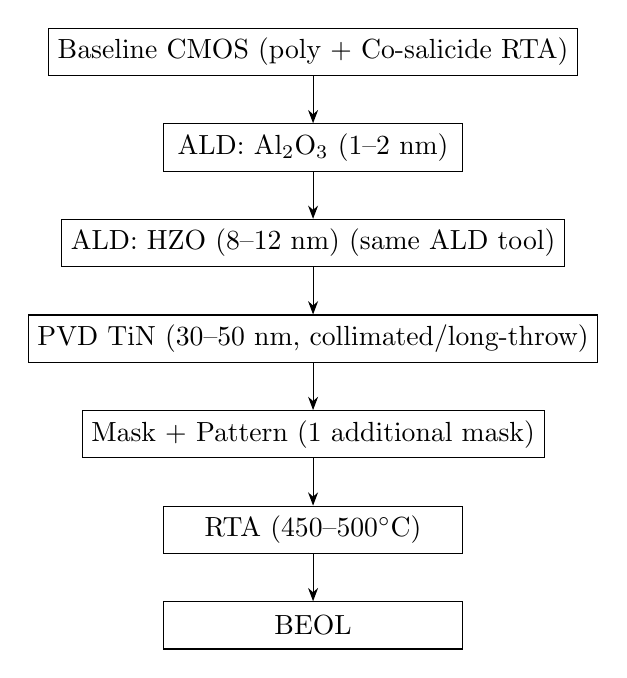
\begin{tikzpicture}[node distance=6mm, every node/.style={draw,rectangle,minimum width=38mm,minimum height=6mm},>=Stealth]
    \node (a) {Baseline CMOS (poly + Co-salicide RTA)};
    \node (b) [below=of a] {ALD: Al$_2$O$_3$ (1--2 nm)};
    \node (c) [below=of b] {ALD: HZO (8--12 nm) (same ALD tool)};
    \node (d) [below=of c] {PVD TiN (30--50 nm, collimated/long-throw)};
    \node (e) [below=of d] {Mask + Pattern (1 additional mask)};
    \node (f) [below=of e] {RTA (450--500$^\circ$C)};
    \node (g) [below=of f] {BEOL};
    \draw[->] (a) -- (b);
    \draw[->] (b) -- (c);
    \draw[->] (c) -- (d);
    \draw[->] (d) -- (e);
    \draw[->] (e) -- (f);
    \draw[->] (f) -- (g);
  \end{tikzpicture}
  \caption{Process flow of FeFET integration after Co-salicide. Only one mask and a single ALD tool are required.}
  \label{fig:flow}
\end{figure}

\subsection{Cross Section}
\begin{figure}[!htb]
  \centering
  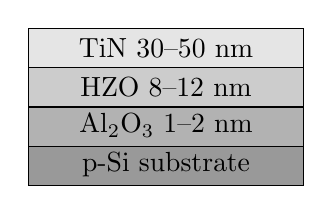
\begin{tikzpicture}
    \node[draw,fill=gray!80,minimum width=35mm,minimum height=5mm,anchor=south west] (si) at (0,0) {p-Si substrate};
    \node[draw,fill=gray!60,minimum width=35mm,minimum height=5mm,anchor=south west] (al) at (0,0.5) {Al$_2$O$_3$ 1--2 nm};
    \node[draw,fill=gray!40,minimum width=35mm,minimum height=5mm,anchor=south west] (hzo) at (0,1.0) {HZO 8--12 nm};
    \node[draw,fill=gray!20,minimum width=35mm,minimum height=5mm,anchor=south west] (tin) at (0,1.5) {TiN 30--50 nm};
  \end{tikzpicture}
  \caption{Cross section of HZO/Al$_2$O$_3$/TiN stack.}
  \label{fig:stack}
\end{figure}

\FloatBarrier

% ========= Devices and Methods =========
\section{Devices and Methods}
\begin{table}[!htb]
  \centering
  \caption{Reliability test matrix (devices: FeCAP/FeFET).}
  \label{tab:test-matrix}
  \begin{tabular}{@{}ll@{}}
    \toprule
    \textbf{Item} & \textbf{Conditions} \\
    \midrule
    TZDB     & DC ramp $\approx 0.1$ V/s,\ RT--\SI{125}{\celsius} \\
    TDDB     & $\pm$2.3/2.5/2.7 V,\ \SI{85}{\celsius}, \SI{125}{\celsius} \\
    Endurance& $\pm$2.5 V,\ \SI{10}{\micro\second},\ \SI{10}{\kilo\hertz}, up to $10^5$ \\
    Retention& \SI{25}{\celsius}, \SI{85}{\celsius}, \SI{125}{\celsius} \\
    \bottomrule
  \end{tabular}
\end{table}

Test structures include FeCAPs (flat/comb) and $100~\mu\mathrm{m}\times100~\mu\mathrm{m}$ FeFET cells.
Programming used $\pm$2.3--2.7~V, 1--50~$\mu$s pulses.
A Keysight B1500A with a manual probe station was used.

\textbf{Protocols}: 
TZDB: DC ramp $\approx 0.1$~V/s at RT--125$^\circ$C.
TDDB: constant-voltage stress at $\pm$2.3/2.5/2.7~V, 85$^\circ$C and 125$^\circ$C; Weibull fitting.
Endurance: $\pm$2.5~V, 10~$\mu$s, 10~kHz up to $10^5$ cycles.
Retention: 25$^\circ$C, 85$^\circ$C, 125$^\circ$C with Arrhenius extrapolation.

\FloatBarrier

% ========= Results (Reliability) =========
\section{Results: Reliability}

\subsection{Time-Zero Dielectric Breakdown (TZDB)}
\begin{figure}[!htb]
  \centering
  \includegraphics[width=\figw]{figures/fig3_tzdb.png}
  \caption{TZDB distributions of FeCAPs. Early-failure tails imply defect-driven breakdown paths.}
  \label{fig:tzdb}
\end{figure}

\subsection{TDDB under Constant-Voltage Stress}
\begin{figure}[!htb]
  \centering
  \includegraphics[width=\figw]{figures/fig4_tddb_cdf.png}
  \caption{TDDB cumulative failure probability (CDF) under multiple stress conditions.}
  \label{fig:tddb_cdf}
\end{figure}

\begin{figure}[!htb]
  \centering
  \includegraphics[width=\figw]{figures/fig4_tddb_weibull.png}
  \caption{TDDB Weibull plots with fitted slope $\beta \approx 1.3$ and scale $\eta$.}
  \label{fig:tddb_weibull}
\end{figure}

\subsection{Endurance}
\begin{figure}[!htb]
  \centering
  \includegraphics[width=\figw]{figures/fig5_endurance.png}
  \caption{Endurance characteristics ($\Delta V_{\mathrm{th}}$ vs. cycles). Up to $10^5$ cycles; memory window shrinks 20--30\%.}
  \label{fig:endurance}
\end{figure}

\subsection{Retention}
\begin{figure}[!htb]
  \centering
  \includegraphics[width=\figw]{figures/fig6_retention.png}
  \caption{Retention summary (CDF and/or Arrhenius extrapolation).}
  \label{fig:retention}
\end{figure}

\subsection{Model Fits}
Time-to-failure follows a Weibull law:
\begin{equation}
  F(t)=1-\exp\!\left[-\left(\frac{t}{\etaW}\right)^{\betaW}\right],
\end{equation}
with slope $\betaW \approx 1.3$ and scale $\etaW$ extracted from Fig.~\ref{fig:tddb_weibull}.
Temperature acceleration is described by an Arrhenius relation:
\begin{equation}
  \ln\!\left(\frac{t_2}{t_1}\right)=\frac{\Ea}{k}\!\left(\frac{1}{T_2}-\frac{1}{T_1}\right).
\end{equation}
Activation energies: $\Ea \approx 0.78$~eV (2.3 V), 0.84 eV (2.5 V), 0.88 eV (2.7 V).  
Endurance fit:
\begin{equation}
  \Delta \Vth(N) \approx 1.12 - 0.05\log_{10} N.
\end{equation}

\subsection*{Summary of Reliability Results}
Fabricated FeFET devices show endurance exceeding $10^5$ cycles (Fig.~\ref{fig:endurance}) and retention $>10$ years at 85$^\circ$C (Fig.~\ref{fig:retention}).  
These results validate the proposed +1 mask integration scheme for automotive and industrial NVM.

\FloatBarrier

% ========= System Architecture =========
\section{System Architecture (SRAM + FeFET)}
The SoC uses a single 1.8~V core domain for logic, SRAM, and FeFET access.
Write/erase pulses are generated by an on-chip charge pump.  
A lightweight controller backs up SRAM contents to the FeFET array on power-fail detection and restores them at power-up.  
An optional 3.3~V domain is kept for I/O and AMS.

Unlike stand-alone high-density NVM, the FeFET array plays a supplementary role as backup/assistive memory for SRAM.  

\begin{figure}[!htb]
  \centering
  \resizebox{0.90\columnwidth}{!}{%
    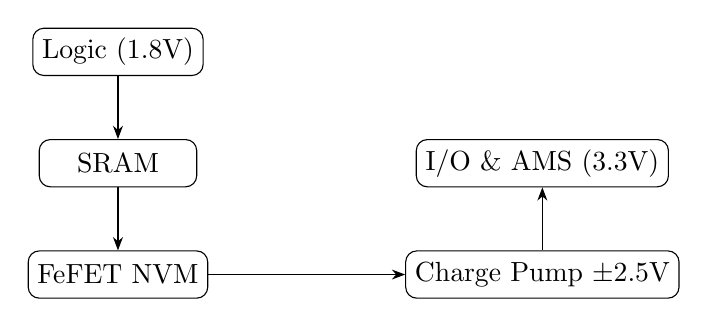
\begin{tikzpicture}[node distance=8mm,
      every node/.style={draw,rounded corners,minimum width=20mm,minimum height=6mm,align=center},
      >=Stealth,transform shape]
      \node (logic) {Logic (1.8V)};
      \node (sram)  [below=of logic] {SRAM};
      \node (fefet) [below=of sram]  {FeFET NVM};
      \node (pump)  [right=25mm of fefet] {Charge Pump $\pm$2.5V};
      \node (io)    [above=of pump] {I/O \& AMS (3.3V)};
      \draw[->] (logic) -- (sram);
      \draw[->] (sram)  -- (fefet);
      \draw[->] (fefet) -- (pump);
      \draw[->] (pump)  -- (io);
    \end{tikzpicture}%
  }
  \caption{System architecture with SRAM backup to FeFET.}
\end{figure}

\begin{figure}[!htb]
  \centering
  \resizebox{0.90\columnwidth}{!}{%
    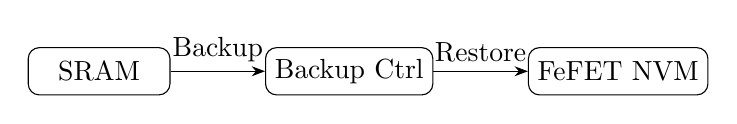
\begin{tikzpicture}[node distance=8mm,
      box/.style={draw,rounded corners,minimum width=18mm,minimum height=6mm},
      >=Stealth,transform shape]
      \node[box] (sram) {SRAM};
      \node[box, right=12mm of sram] (ctrl) {Backup Ctrl};
      \node[box, right=12mm of ctrl] (nvm)  {FeFET NVM};
      \draw[-{Stealth}] (sram) -- node[above,sloped]{Backup}  (ctrl);
      \draw[-{Stealth}] (ctrl) -- node[above,sloped]{Restore} (nvm);
    \end{tikzpicture}%
  }
  \caption{Backup/restore flow between SRAM and FeFET.}
\end{figure}

\FloatBarrier

% ========= Discussion =========
\section{Discussion}
The HfZrO$_2$/Al$_2$O$_3$/TiN stack shows sufficient reliability for embedded NVM.  
For high-temperature automotive, improvements are required:
\begin{itemize}
  \item \textbf{Interlayer optimization}: Al$_2$O$_3$ thickness tuning.
  \item \textbf{Crystallinity control}: RTA window and TiN work-function.
  \item \textbf{Defect mitigation}: Precursor purity, ALD purge, post-anneal.
  \item \textbf{Circuit assists}: ECC, adaptive pulses, refresh. 
  \item \textbf{Array architecture}: Redundancy/repair, SRAM+FeFET hybrid.
\end{itemize}

The FeFET’s role as SRAM backup (not stand-alone NVM) avoids density stress, improves yield, and enhances reliability for industrial/automotive.

\FloatBarrier

% ========= Conclusion =========
\section{Conclusion}
We demonstrated a +1 mask FeFET module on 0.18~$\mu$m CMOS, requiring only one ALD tool.  
Devices achieved endurance $>10^5$ cycles and retention $>10$ years at 85$^\circ$C, verified by TZDB, TDDB, endurance and retention analyses.  
Positioning the FeFET array as a supplementary backup to SRAM—rather than a stand-alone high-density NVM—reduces scaling pressure, improves yield, and enhances reliability for automotive, industrial, and IoT applications.  
Overall, the method provides a cost-effective path to extend mature-node lifetimes while delivering dependable embedded nonvolatile memory.

\FloatBarrier

% ========= Acknowledgment =========
\section*{Acknowledgment}
The author thanks collaborators for helpful discussions.

% ========= References =========
\begin{thebibliography}{1}\setlength{\itemsep}{0pt plus 0.3pt}
\bibitem{boscke2011} T. Böscke \textit{et al.}, \textit{Appl. Phys. Lett.}, vol. 99, p. 102903, 2011.
\bibitem{mueller2012} J. Müller \textit{et al.}, \textit{Appl. Phys. Lett.}, vol. 99, p. 112901, 2012.
\bibitem{mikolajick2019} T. Mikolajick \textit{et al.}, \textit{J. Appl. Phys.}, vol. 125, p. 204103, 2019.
\bibitem{mueller2015} J. Müller \textit{et al.}, \textit{IEEE Trans. Electron Devices}, vol. 62, no. 12, pp. 4158--4166, 2015.
\bibitem{park2020} J. Park \textit{et al.}, \textit{IEEE Electron Device Lett.}, vol. 41, no. 5, pp. 711--714, 2020.
\bibitem{nakamura2003} H. Nakamura \textit{et al.}, \textit{IEEE Trans. Device Mater. Rel.}, vol. 3, no. 4, pp. 132--136, 2003.
\bibitem{yamazaki2018} K. Yamazaki \textit{et al.}, \textit{Jpn. J. Appl. Phys.}, vol. 57, 04FB07, 2018.
\end{thebibliography}

% ========= Biography =========
\section*{Biography}
\small
Shinichi Samizo has over 25 years of experience in semiconductor process integration and actuator development. After studying control theory and EM modeling in academia, he joined Seiko Epson in 1997 and worked on 0.35--0.18~$\mu$m CMOS logic/memory/HV integration, DRAM, and LCD drivers. Later he contributed to PZT actuator development and the PrecisionCore inkjet head. He is currently an independent researcher, publishing educational materials via the ``Project Design Hub''.

\end{document}
